\begin{figure}[t]
\centering
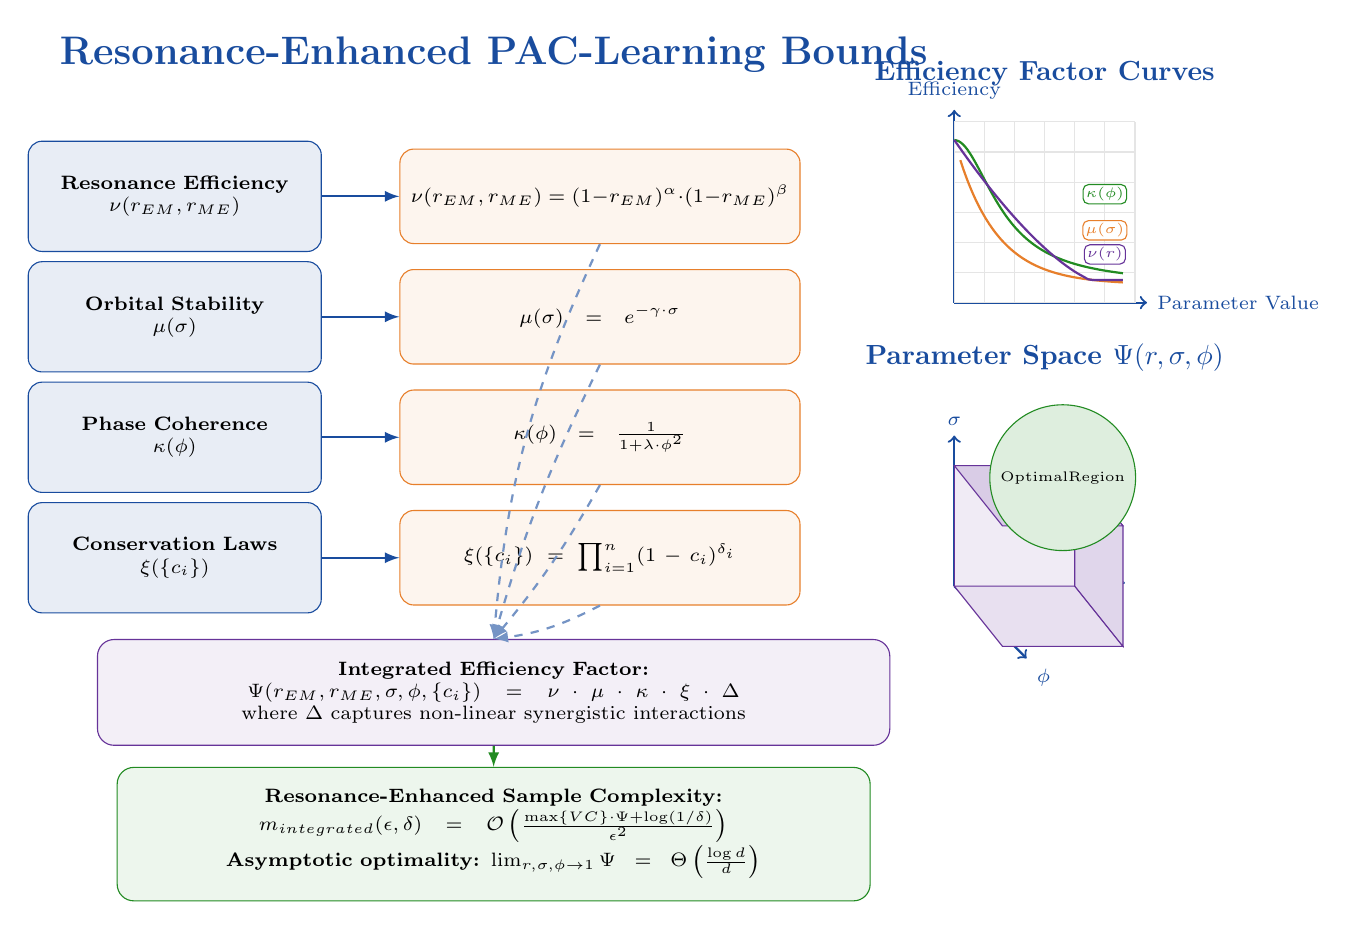
\begin{tikzpicture}[scale=0.9]
    % Define Elder color palette
    \definecolor{elderblue}{RGB}{25,76,158}
    \definecolor{elderorange}{RGB}{231,127,43}
    \definecolor{eldergreen}{RGB}{34,139,34}
    \definecolor{elderpurple}{RGB}{102,51,153}
    
    % Define clean, modern styles
    \tikzset{
        factor/.style={
            draw=elderblue,
            fill=elderblue!10,
            rounded corners=5pt,
            minimum width=3.5cm,
            minimum height=1.4cm,
            text width=3.3cm,
            align=center,
            font=\scriptsize,
            inner sep=6pt
        },
        equation/.style={
            draw=elderorange,
            fill=elderorange!8,
            rounded corners=5pt,
            minimum width=5cm,
            minimum height=1.2cm,
            text width=4.8cm,
            align=center,
            font=\scriptsize,
            inner sep=4pt
        },
        arrow/.style={
            ->,
            elderblue,
            thick,
            >=latex
        },
        result/.style={
            draw=eldergreen,
            fill=eldergreen!8,
            rounded corners=6pt,
            text width=9cm,
            align=center,
            font=\scriptsize,
            inner sep=8pt
        }
    }
    
    % Title with better spacing
    \node[font=\Large\bfseries, elderblue] at (4.5,8.5) {Resonance-Enhanced PAC-Learning Bounds};
    
    % Left column: Efficiency factors with better spacing
    \node[factor] (res) at (0,6.5) {\textbf{Resonance Efficiency}\\$\nu(r_{EM}, r_{ME})$};
    \node[factor] (orb) at (0,4.8) {\textbf{Orbital Stability}\\$\mu(\sigma)$};
    \node[factor] (phase) at (0,3.1) {\textbf{Phase Coherence}\\$\kappa(\phi)$};
    \node[factor] (cons) at (0,1.4) {\textbf{Conservation Laws}\\$\xi(\{c_i\})$};
    
    % Right column: Mathematical expressions with cleaner layout
    \node[equation] (eq_res) at (6,6.5) {$\nu(r_{EM}, r_{ME}) = (1 - r_{EM})^{\alpha} \cdot (1 - r_{ME})^{\beta}$};
    \node[equation] (eq_orb) at (6,4.8) {$\mu(\sigma) = e^{-\gamma \cdot \sigma}$};
    \node[equation] (eq_phase) at (6,3.1) {$\kappa(\phi) = \frac{1}{1 + \lambda \cdot \phi^2}$};
    \node[equation] (eq_cons) at (6,1.4) {$\xi(\{c_i\}) = \prod_{i=1}^{n} (1 - c_i)^{\delta_i}$};
    
    % Integrated factor with improved design
    \node[draw=elderpurple, fill=elderpurple!8, rounded corners=6pt, text width=9.5cm, align=center, font=\scriptsize, inner sep=8pt] (integrated) at (4.5,-0.5) {
        \textbf{Integrated Efficiency Factor:}\\
        $\Psi(r_{EM}, r_{ME}, \sigma, \phi, \{c_i\}) = \nu \cdot \mu \cdot \kappa \cdot \xi \cdot \Delta$\\
        where $\Delta$ captures non-linear synergistic interactions
    };
    
    % Clean connections between factors and equations
    \draw[arrow] (res) -- (eq_res);
    \draw[arrow] (orb) -- (eq_orb);
    \draw[arrow] (phase) -- (eq_phase);
    \draw[arrow] (cons) -- (eq_cons);
    
    % Cleaner convergence to integrated factor
    \draw[arrow, elderblue!60, dashed] (eq_res.south) to[bend right=10] (integrated.north);
    \draw[arrow, elderblue!60, dashed] (eq_orb.south) to[bend right=5] (integrated.north);
    \draw[arrow, elderblue!60, dashed] (eq_phase.south) to[bend left=5] (integrated.north);
    \draw[arrow, elderblue!60, dashed] (eq_cons.south) to[bend left=10] (integrated.north);
    
    % Final sample complexity result
    \node[result] (complexity) at (4.5,-2.5) {
        \textbf{Resonance-Enhanced Sample Complexity:}\\
        $m_{integrated}(\epsilon, \delta) = \mathcal{O}\left(\frac{\max\{\text{VC}\} \cdot \Psi + \log(1/\delta)}{\epsilon^2}\right)$\\
        \textbf{Asymptotic optimality:} $\lim_{r, \sigma, \phi \to 1} \Psi = \Theta\left(\frac{\log d}{d}\right)$
    };
    
    \draw[arrow, eldergreen, thick] (integrated) -- (complexity);
    
    % Efficiency curves visualization
    \begin{scope}[shift={(11,5)}, scale=0.85]
        % Title
        \node[font=\normalsize\bfseries, elderblue] at (1.5,3.8) {Efficiency Factor Curves};
        
        % Cleaner coordinate system
        \draw[thick, elderblue, ->] (0,0) -- (3.2,0) node[right, font=\scriptsize] {Parameter Value};
        \draw[thick, elderblue, ->] (0,0) -- (0,3.2) node[above, font=\scriptsize] {Efficiency};
        
        % Grid for better readability
        \draw[gray!20] (0,0) grid[step=0.5] (3,3);
        
        % Efficiency curves with Elder colors
        \draw[domain=0.1:2.8, samples=40, smooth, variable=\x, elderorange, thick] 
            plot ({\x}, {0.3 + 2.4 * exp(-1.5*\x)});
        \draw[domain=0:2.8, samples=40, smooth, variable=\x, eldergreen, thick] 
            plot ({\x}, {0.3 + 2.4 / (1 + 1.5*\x*\x)});
        \draw[domain=0:2.8, samples=40, smooth, variable=\x, elderpurple, thick] 
            plot ({\x}, {0.3 + 2.4 * pow(max(1-\x/2.5,0.1), 1.5)});
        
        % Better curve labels
        \node[elderorange, fill=white, draw=elderorange, rounded corners=2pt, font=\tiny, inner sep=1pt] at (2.5,1.2) {$\mu(\sigma)$};
        \node[eldergreen, fill=white, draw=eldergreen, rounded corners=2pt, font=\tiny, inner sep=1pt] at (2.5,1.8) {$\kappa(\phi)$};
        \node[elderpurple, fill=white, draw=elderpurple, rounded corners=2pt, font=\tiny, inner sep=1pt] at (2.5,0.8) {$\nu(r)$};
    \end{scope}
    
    % Simplified 3D parameter space visualization
    \begin{scope}[shift={(11,1)}, scale=0.85]
        % Title
        \node[font=\normalsize\bfseries, elderblue] at (1.5,3.8) {Parameter Space $\Psi(r, \sigma, \phi)$};
        
        % Clean 3D axes
        \draw[thick, elderblue, ->] (0,0) -- (2.5,0) node[right, font=\scriptsize] {$r$};
        \draw[thick, elderblue, ->] (0,0) -- (0,2.5) node[above, font=\scriptsize] {$\sigma$};
        \draw[thick, elderblue, ->] (0,0) -- (1.2,-1.2) node[below right, font=\scriptsize] {$\phi$};
        
        % Clean surface representation
        \draw[fill=elderpurple!10, draw=elderpurple] (0,0) -- (2,0) -- (2,2) -- (0,2) -- cycle;
        \draw[fill=elderpurple!15, draw=elderpurple] (0,0) -- (2,0) -- (2.8,-1) -- (0.8,-1) -- cycle;
        \draw[fill=elderpurple!20, draw=elderpurple] (2,0) -- (2.8,-1) -- (2.8,1) -- (2,2) -- cycle;
        \draw[fill=elderpurple!25, draw=elderpurple] (0,2) -- (2,2) -- (2.8,1) -- (0.8,1) -- cycle;
        
        % Optimal region indicator
        \node[draw=eldergreen, fill=eldergreen!15, circle, minimum size=0.8cm, font=\tiny] at (1.8,1.8) {Optimal\\Region};
    \end{scope}
    
\end{tikzpicture}
\caption{Resonance-enhanced PAC-learning bounds for Elder systems. The sample complexity is determined by four key efficiency factors: the resonance efficiency $\nu(r_{EM}, r_{ME})$, which depends on the resonance strength between hierarchical levels; the orbital stability factor $\mu(\sigma)$, which captures the impact of stable orbits on learning efficiency; the phase coherence factor $\kappa(\phi)$, which quantifies the benefits of synchronized learning trajectories; and the conservation law factor $\xi(\{c_i\})$, which accounts for the constraints imposed by conserved quantities. These factors combine through the integrated efficiency factor $\Psi$, which includes non-linear interactions captured by the synergy factor $\Delta$. Under optimal conditions, the integrated factor approaches $\Theta(\frac{\log d}{d})$, providing asymptotic improvement beyond the standard logarithmic efficiency gain.}
\label{fig:resonance_pac}
\end{figure}